\section{Introduction to Embedded Linux}

\begin{frame}
  \frametitle{Birth of Free Software}
  \begin{columns}
    \column{0.75\textwidth}
      \begin{itemize}
      \item 1983, Richard Stallman, {\bf GNU project} and the {\bf free
          software} concept.  Beginning of the development of {\em gcc},
        {\em gdb}, {\em glibc} and other important tools
      \item 1991, Linus Torvalds, {\bf Linux kernel project}, a UNIX-like
        operating system kernel. Together with GNU software and many other
        open-source components: a completely free operating system,
        GNU/Linux
      \item ~1995, Linux is more and more popular on server systems
      \item ~2000, Linux is more and more popular on {\bf embedded
          systems}
      \item ~2008, Linux is more and more popular on mobile devices and phones
      \item ~2012, Linux is available on cheap, extensible hardware:
            Raspberry Pi, BeagleBone Black
      \end{itemize}
    \column{0.25\textwidth}
      \includegraphics[width=\textwidth]{slides/sysdev-intro/richard-stallman.jpg}
      \scriptsize
      Richard Stallman in 2019\\
      \tiny
      Image credits (Wikipedia):\\
      \url{https://frama.link/qC73jkk4}
    \end{columns}

\end{frame}

\begin{frame}
  \frametitle{Free software?}
  \begin{itemize}
  \item A program is considered {\bf free} when its license offers to
    all its users the following {\bf four} freedoms
    \begin{itemize}
    \item Freedom to run the software for any purpose
    \item Freedom to study the software and to change it
    \item Freedom to redistribute copies
    \item Freedom to distribute copies of modified versions
    \end{itemize}
  \item These freedoms are granted for both commercial and
    non-commercial use
  \item They imply the availability of source code, software can be
    modified and distributed to customers
  \item {\bf Good match for embedded systems!}
  \end{itemize}
\end{frame}

\begin{frame}{What is embedded Linux?}
  \huge
  \begin{center}
    Embedded Linux is the usage of the {\bf Linux kernel} and various
    {\bf open-source} components in embedded systems
  \end{center}
\end{frame}

\subsection[Why embedded Linux?]{Advantages of Linux and open-source
  for embedded systems}

\begin{frame}
  \frametitle{Re-using components}
  \begin{itemize}
  \item The key advantage of Linux and open-source in embedded systems
    is the {\bf ability} to re-use components
  \item The open-source ecosystem already provides many components for
    standard features, from hardware support to network protocols,
    going through multimedia, graphic, cryptographic libraries, etc.
  \item As soon as a hardware device, or a protocol, or a feature is
    wide-spread enough, high chance of having open-source components
    that support it.
  \item Allows to quickly design and develop complicated products,
    based on existing components.
  \item No-one should re-develop yet another operating system kernel,
    TCP/IP stack, USB stack or another graphical toolkit library.
  \item {\bf Allows to focus on the added value of your product.}
  \end{itemize}
\end{frame}

\begin{frame}
  \frametitle{Low cost}
  \begin{itemize}
  \item Free software can be duplicated on as many devices as you
    want, free of charge.
  \item If your embedded system uses only free software, you can
    reduce the cost of software licenses to zero. Even the development
    tools are free, unless you choose a commercial embedded Linux
    edition.
  \item Of course, using Linux is not free of cost. You still need
    substantial learning and engineering efforts to achieve your
    goals.
  \item {\bf Allows to have a higher budget for the hardware or to
      increase the company’s skills and knowledge}
  \end{itemize}
\end{frame}

\begin{frame}
  \frametitle{Full control}
  \begin{itemize}
  \item With open-source, you have the source code for all components
    in your system
  \item Allows unlimited modifications, changes, tuning, debugging,
    optimization, for an unlimited period of time
  \item Without lock-in or dependency from a third-party vendor
    \begin{itemize}
    \item To be true, non open-source components must be avoided when
      the system is designed and developed
    \end{itemize}
  \item {\bf Allows to have full control over the software part of
      your system and secure your investment}
  \end{itemize}
\end{frame}

\begin{frame}
  \frametitle{Quality}
  \begin{itemize}
  \item Many open-source components are widely used, on millions of
    systems
  \item Usually higher quality than what an in-house development can
    produce, or even proprietary vendors
  \item Of course, not all open-source components are of good quality,
    but most of the widely-used ones are.
  \item {\bf Allows to design your system with high-quality components
      at the foundations}
\end{itemize}
\end{frame}

\begin{frame}
  \frametitle{Eases testing of new features}
  \begin{itemize}
  \item Open-source being freely available, it is easy to get a piece
    of software and evaluate it
  \item Allows to easily study several options while making a choice
  \item Much easier than purchasing and demonstration procedures
    needed with most proprietary products
  \item {\bf Allows to easily explore new possibilities and solutions}
  \end{itemize}
\end{frame}

\begin{frame}
  \frametitle{Community support}
  \begin{itemize}
  \item Open-source software components are developed by communities
    of developers and users
  \item This community can provide high-quality support: you can
    directly contact the main developers of the component you are
    using. The likelihood of getting an answer doesn't depend what
    company you work for.
  \item Often better than traditional support, but one needs to
    understand how the community works to properly use the community
    support possibilities
  \item {\bf Allows to speed up the resolution of problems when
      developing your system}
  \end{itemize}
\end{frame}

\begin{frame}
  \frametitle{Taking part into the community}
  \begin{itemize}
  \item Possibility of taking part into the development community of
    some of the components used in the embedded systems: bug
    reporting, test of new versions or features, patches that fix bugs
    or add new features, etc.
  \item Most of the time the open-source components are not the core
    value of the product: it’s the interest of everybody to contribute
    back.
  \item For the {\em engineers}: a very {\bf motivating} way of being
    recognized outside the company, communication with others in the
    same field, {\bf opening of new possibilities}, etc.
  \item For the {\em managers}: {\bf motivation factor} for engineers,
    allows the company to be {\bf recognized} in the open-source
    community and therefore get support more easily and be {\bf more
      attractive} to open-source developers
\end{itemize}
\end{frame}

\subsection[Systems running Linux]{A few examples of embedded systems
  running Linux}

\begin{frame}
  \frametitle{Wireless routers}
  \begin{center}
    \includegraphics[height=0.8\textheight]{slides/sysdev-intro/linksys-wireless-router.jpg}
  \end{center}
  \tiny
  Image credits: Evan Amos (\url{https://bit.ly/2JzDIkv})
\end{frame}

\begin{frame}
\frametitle{Video systems}
  \begin{center}
    \includegraphics[height=0.8\textheight]{slides/sysdev-intro/chromecast-2015.jpg}
  \end{center}
  \tiny Image credits: \url{https://bit.ly/2HbwyVq}
\end{frame}

\begin{frame}
\frametitle{Bike computers}
  \begin{center}
    \includegraphics[height=0.8\textheight]{slides/sysdev-intro/bike-computer.jpg}
  \end{center}
  \tiny
  Product from BLOKS (\url{http://bloks.de}).
  Permission to use this picture only in this document, in updates and
  in translations.
\end{frame}

\begin{frame}
\frametitle{Robots}
  \begin{center}
    \includegraphics[height=0.75\textheight]{slides/sysdev-intro/beagle-robot.jpg}
  \end{center}
  eduMIP robot (\url{https://www.ucsdrobotics.org/edumip})
\end{frame}

\begin{frame}
\frametitle{In space}
  \small
  \begin{columns}
  \column{0.5\textwidth}
  SpaceX Starlink satelites\\
  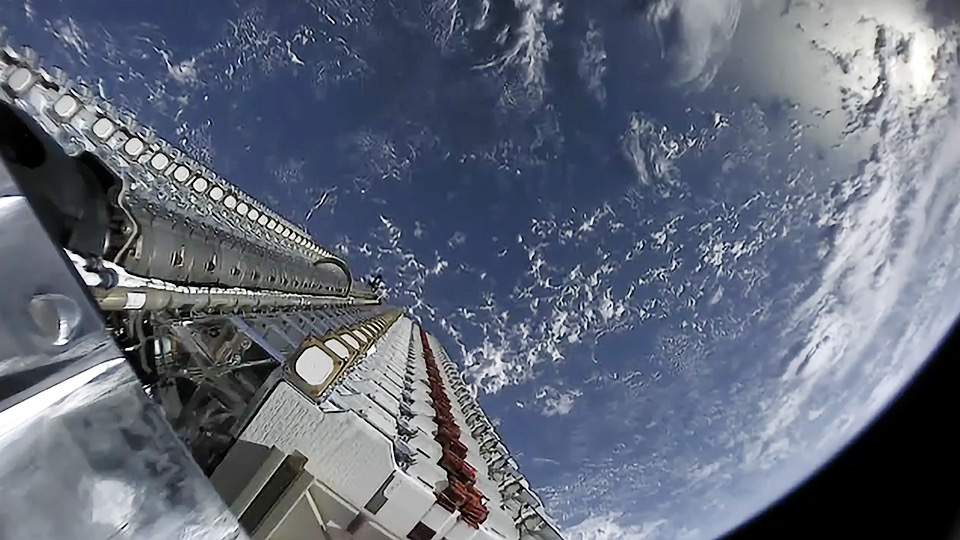
\includegraphics[height=0.35\textheight]{slides/sysdev-intro/starlink.jpg}\\
  SpaceX Falcon 9 and Falcon Heavy rockets\\
  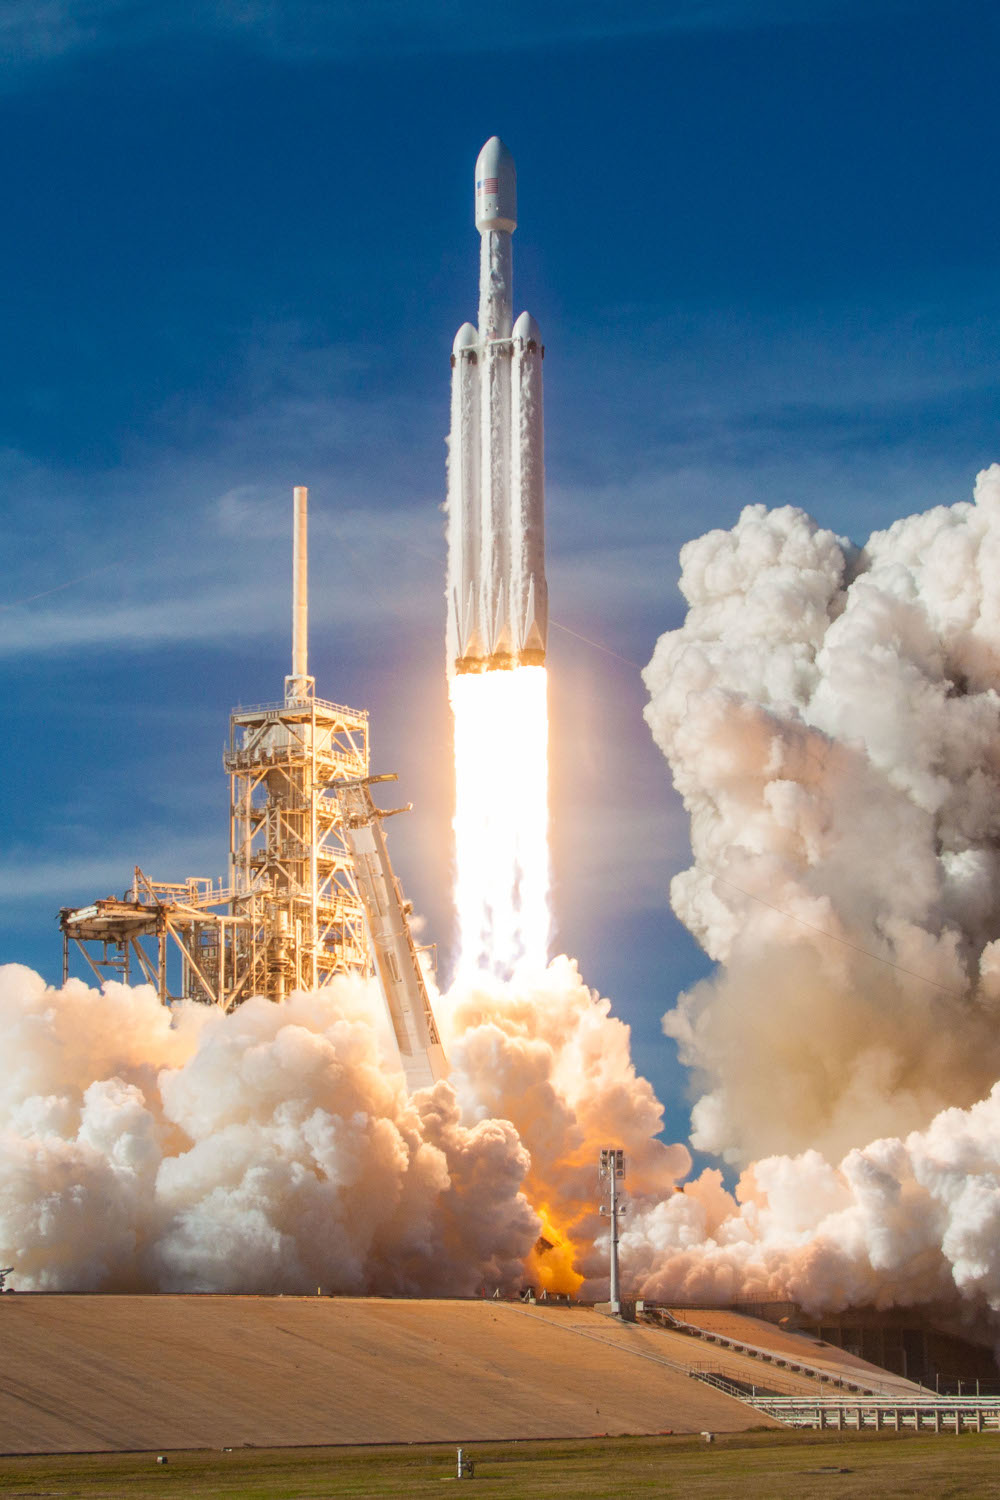
\includegraphics[height=0.35\textheight]{slides/sysdev-intro/falcon-heavy.jpg}\\
  \column{0.5\textwidth}
  Mars Ingenuity Helicopter\\
  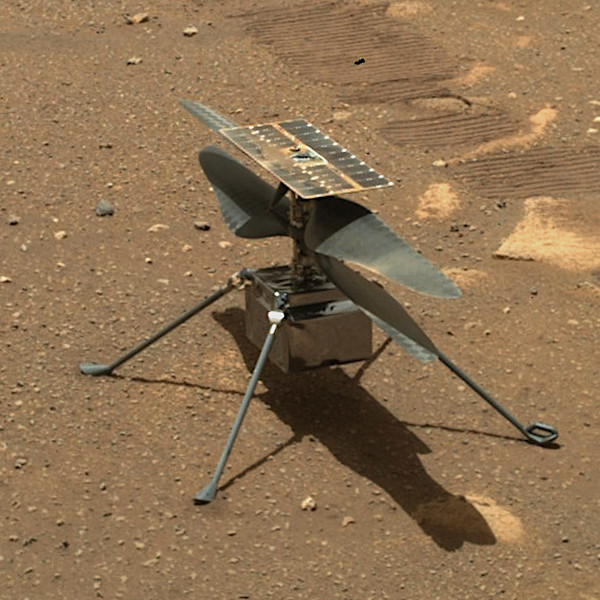
\includegraphics[height=0.35\textheight]{slides/sysdev-intro/mars-helicopter.jpg}\\
  \vspace{3cm}
  \tiny Image credits: Wikipedia
  \end{columns}
\end{frame}

\subsection{Embedded hardware for Linux systems}

\begin{frame}
  \frametitle{Processor and architecture (1)}
  The Linux kernel and most other architecture-dependent
  components support a wide range of 32 and 64 bit architectures
  \begin{itemize}
  \item x86 and x86-64, as found on PC platforms, but also embedded systems
    (multimedia, industrial)
  \item ARM, with hundreds of different {\em System on Chip}s\\
        ({\em SoC}: CPU + on-chip devices, for all sorts of products)
  \item RISC-V, the rising architecture with a free instruction set\\
        (from high-end cloud computing to the smallest embedded systems)
  \item PowerPC (mainly real-time, industrial applications)
  \item MIPS (mainly networking applications)
  \item Microblaze (Xilinx), Nios II (Altera): soft cores on FPGAs
  \item Others: ARC, m68k, Xtensa, SuperH...
  \end{itemize}
\end{frame}

\begin{frame}
  \frametitle{Processor and architecture (2)}
  \begin{itemize}
  \item Both MMU and no-MMU architectures are supported, even though
    no-MMU architectures have a few limitations.
  \item Linux does not support small microcontrollers (8 or 16 bit)
  \item Besides the toolchain, the bootloader and the kernel, all
    other components are generally {\bf architecture-independent}
  \end{itemize}
\end{frame}

\begin{frame}
  \frametitle{RAM and storage}
  \begin{itemize}
  \item {\bf RAM}: a very basic Linux system can work within 8 MB of
    RAM, but a more realistic system will usually require at least 32
    MB of RAM. Depends on the type and size of applications.
  \item {\bf Storage}: a very basic Linux system can work within 4 MB
    of storage, but usually more is needed.
    \begin{itemize}
    \item {\bf Block storage}: SD/MMC/eMMC, USB mass storage, SATA, etc,
    \item {\bf Raw flash storage} is supported too, both NAND and NOR flash, with
      specific filesystems
    \end{itemize}
  \item Not necessarily interesting to be too restrictive on the
    amount of RAM/storage: having flexibility at this level allows to
    re-use as many existing components as possible.
  \end{itemize}
\end{frame}

\begin{frame}
  \frametitle{Communication}
  \begin{itemize}
  \item The Linux kernel has support for many common communication
    buses
    \begin{itemize}
    \item I2C
    \item SPI
    \item 1-wire
    \item SDIO
    \item PCI
    \item USB
    \item CAN (mainly used in automotive)
    \end{itemize}
  \item And also extensive networking support
    \begin{itemize}
    \item Ethernet, Wifi, Bluetooth, CAN, etc.
    \item IPv4, IPv6, TCP, UDP, SCTP, DCCP, etc.
    \item Firewalling, advanced routing, multicast
    \end{itemize}
  \end{itemize}
\end{frame}

\begin{frame}
  \frametitle{Types of hardware platforms (1)}
  \begin{columns}
  \column{0.75\textwidth}
  \begin{itemize}
  \item {\bf Evaluation platforms} from the SoC vendor. Usually
    expensive, but many peripherals are built-in. Generally unsuitable
    for real products, but best for product development.
  \item {\bf Component on Module}, a small board with only
    CPU/RAM/flash and a few other core components, with connectors to
    access all other peripherals. Can be used to build end products
    for small to medium quantities.
  \end{itemize}
  \column{0.25\textwidth}
    \includegraphics[width=\textwidth]{slides/sysdev-intro/stm32mp157c-ev1.png}
    \scriptsize
    STM32MP157C-EV1 evaluation board\\
    \tiny
    Image credits (st.com):\\
    \url{https://frama.link/NySnaxuV}\\
    \vspace{0.5cm}
    \includegraphics[width=\textwidth]{slides/sysdev-intro/pocketbeagle.png}
    \scriptsize
    PocketBeagle\\
    \tiny
    Image credits (Beagleboard.org):\\
    \url{https://beagleboard.org/pocket}
  \end{columns}
\end{frame}

\begin{frame}
  \frametitle{Types of hardware platforms (2)}
  \begin{columns}
  \column{0.75\textwidth}
  \begin{itemize}
  \item {\bf Community development platforms}, to make a
    particular SoC popular and easily available. These are
    ready-to-use and low cost, but usually have less peripherals than
    evaluation platforms. To some extent, can also be used for real
    products.
  \item {\bf Custom platform}. Schematics for evaluation boards or
    development platforms are more and more commonly freely available,
    making it easier to develop custom platforms.
  \end{itemize}
  \column{0.25\textwidth}
    \includegraphics[height=0.3\textheight]{../slides/beagleboneblack-board/beagleboneblack.png}
    \scriptsize
    Beaglebone Black board\\
    \vspace{0.5cm}
    \includegraphics[height=0.3\textheight]{slides/sysdev-intro/teres-pcb1-a64.jpg}
    \scriptsize
    Olimex Open hardware ARM laptop main board\\
    \tiny
    Image credits (Olimex):\\
    \url{https://www.olimex.com/Products/DIY-Laptop/}
  \end{columns}
\end{frame}

\begin{frame}
  \frametitle{Criteria for choosing the hardware}
  \begin{itemize}
  \item Make sure the hardware you plan to use is already supported by
    the Linux kernel, and has an open-source bootloader, especially
    the SoC you’re targeting.
  \item Having support in the official versions of the projects
    (kernel, bootloader) is a lot better: quality is better, and new
    versions are available.
  \item Some SoC vendors and/or board vendors do not contribute their
    changes back to the mainline Linux kernel. Ask them to do so, or
    use another product if you can. A good measurement is to see the
    delta between their kernel and the official one.
  \item {\bf Between properly supported hardware in the official Linux
      kernel and poorly-supported hardware, there will be huge
      differences in development time and cost.}
  \end{itemize}
\end{frame}

\subsection{Embedded Linux system architecture}

\begin{frame}
  \frametitle{Host and target}
  \begin{center}
    \includegraphics[width=0.9\textwidth]{slides/sysdev-intro/host-and-target.pdf}
  \end{center}
\end{frame}

\begin{frame}
  \frametitle{Software components}
  \begin{itemize}
  \item Cross-compilation toolchain
    \begin{itemize}
    \item Compiler that runs on the development machine, but generates
      code for the target
    \end{itemize}
  \item Bootloader
    \begin{itemize}
    \item Started by the hardware, responsible for basic
      initialization, loading and executing the kernel
    \end{itemize}
  \item Linux Kernel
    \begin{itemize}
    \item Contains the process and memory management, network stack,
      device drivers and provides services to user space applications
    \end{itemize}
  \item C library
    \begin{itemize}
    \item The interface between the kernel and the user space
      applications
    \end{itemize}
  \item Libraries and applications
    \begin{itemize}
    \item Third-party or in-house
    \end{itemize}
  \end{itemize}
\end{frame}

\begin{frame}
  \frametitle{Embedded Linux work}

  Several distinct tasks are needed when deploying embedded Linux in a
  product:

  \begin{itemize}
  \item {\bf Board Support Package development}
    \begin{itemize}
    \item A BSP contains a bootloader and kernel with the suitable
      device drivers for the targeted hardware
    \item Purpose of our \href{https://bootlin.com/training/kernel}
      {\em Kernel Development course}
    \end{itemize}
  \item {\bf System integration}
    \begin{itemize}
    \item Integrate all the components, bootloader, kernel,
      third-party libraries and applications and in-house applications
      into a working system
    \item Purpose of {\em this} course
    \end{itemize}
  \item {\bf Development of applications}
    \begin{itemize}
    \item Normal Linux applications, but using specifically chosen
      libraries
    \end{itemize}
  \end{itemize}
\end{frame}
